
% ---------------------------------------------------
% \section{Spanwise 1D Spectra}
% \section{\label{sec:InnerPeak} Scaling:\protect\\ Inner Peak }
% ---------------------------------------------------

The spanwise power-spectral density of a Reynolds-stress component $\overline{u_iu_j}(y)$ is denoted as $\phi_{u_iu_j}(y,k_z)$, where $k_z$ is the spanwise wavenumber.
% \rev{
% and $y$ is the wall-normal coordinate.
% }
Note that the integral over all the scales is equal to the total RS. Using this property, we can use an integral to determine the marginal contribution of small or large scales to the total RS (marginal contribution of energy, MCE). This can be written as follows:
\begin{equation}
\mathrm{MCE} = \int_{k_{z,c}}^{\infty} \phi_{u_iu_j} \mathrm{d} k_z \ \bigg/ \int_{0}^{\infty} \phi_{u_iu_j} \mathrm{d} k_z,
\label{eq:cumsum}
\end{equation}
where $k_{z,c}$ is the cut-off wavenumber.
The spectra will be analysed through contours of the premultiplied power-spectral density $k_z\phi_{u_iu_j}$ and contours of the marginal contribution to the RS as a percentage. Instead of the wavenumbers $k_z$, the contours will be represented against the spanwise wavelength $\lambda_z=2\pi/k_z$.

The pre-multiplied spanwise spectra of the streamwise RS $k_z\phi_{uu}(y,\lambda_z)$ for both the APG and ZPG clearly show the near-wall and outer spectral peaks, as can be observed below in Fig.~\ref{fig:inner_kPSDz}(a). 
The location of these spectral peaks can be scaled with a length scale to collapse the wall-normal position, here denoted as $y_{s \rm IP}$ and $y_{s \rm OP}$, and another length scale can be used to scale the wavelength of the peaks $\lambda_{z,s \rm IP}$ and $\lambda_{z,s \rm OP}$.
In previous studies, the same scaling factor was used for the wall-normal location and for the wavelength $\lambda_z$; the novelty here is that we allow for a mixed scaling, {\it i.e.} the spanwise structures can have a different scaling than the wall-normal position where they are located, and Fig.~\ref{fig:inner_kPSDz}(b) shows the success of this approach.
A more complex analysis would be to determine the scalings for the energetic contours, since an energy scaling would be required for $k_z\phi_{uu}$, and the contours can be taken at a certain energy level or at a certain percentage of the peak or the maxima. For this last analysis the use of the MCE is useful. 

% \subsection{Peak values of the streamwise spectra}

\begin{figure}
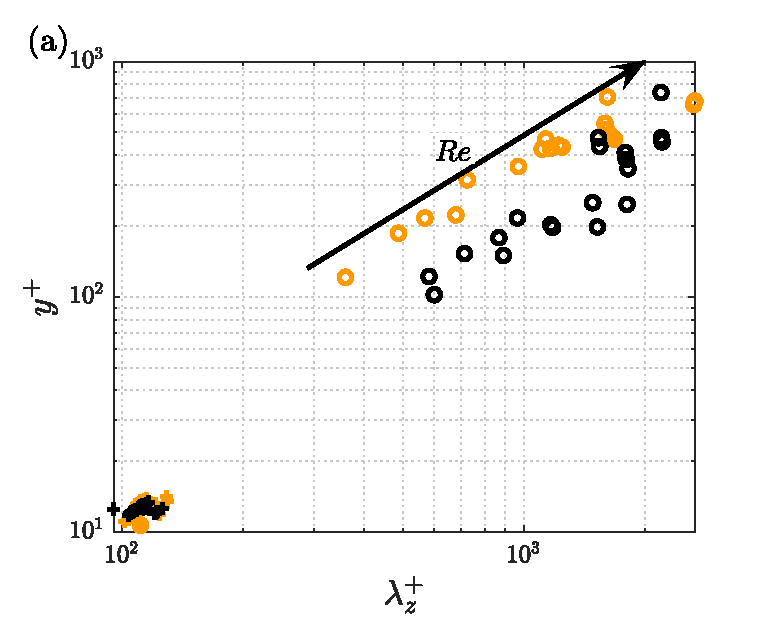
\includegraphics[width=0.49 \textwidth]{peak_uu_ltau_ltau.eps}
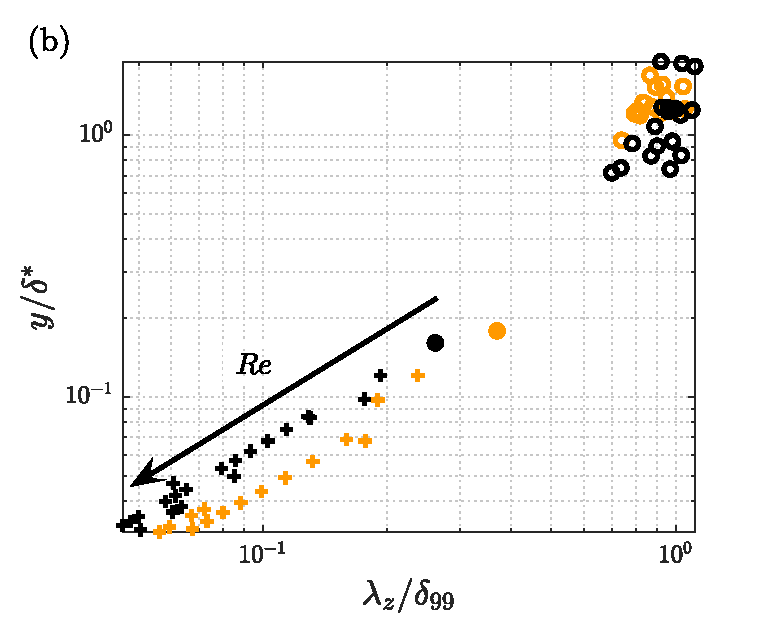
\includegraphics[width=0.49 \textwidth]{peak_uu_dstar_d99.eps}
\caption{ \label{fig:peaks} Representation of the peaks in the premultiplied streamwise power-spectral density $k_z\phi_{uu}$ in (a) inner scaling and (b) scaling with boundary-layer and displacement thicknesses. Crosses denote the inner peak (IP) and circles for the outer peak (OP). Note that in (a) the inner peaks collapse by scaling the wall-normal position $y$ and the wavelength $\lambda_z$ in viscous units, and in (b) the outer peaks collapse when scaling $y$ and $\lambda_z$ with $\delta^*$ and $\delta_{99}$, respectively. The black arrows show the direction of increasing Reynolds number.}
\end{figure}

The near-wall peak of $\overline{u^2}$ is closely connected with the spectral near-wall peak of $k_z\phi_{uu}$, thus it is natural to use the viscous scaling for this region as shown in Fig.~\ref{fig:peaks}(a) for a number of profiles between $Re_{\tau}=1000$ and 2000. This figure shows that the spectral inner peaks are located at approximately the same location for both APG and ZPG, at $y_{s \rm IP}^+\simeq 12.5$, without a clear trend due to the resolution taken for the spectra close to the wall.
The spanwise wavelenghts of the near-wall peak also collapse using inner scaling to a value $\lambda_{z,s \rm IP}^+ \approx 112$.

The outer peak of the RS is related with the spectral outer peak, and Fig.~\ref{fig:peaks}(b) shows that this spectral peak collapses in the premultiplied spectra. In particular, the wall-normal location of the outer peak scales with $\delta^*$ as in Ref.~\cite{Kitsios2017}, while the spanwise wavelength $\lambda_z$ scales with $\delta_{99}$ \cite{Lee2017, bobke2017}. Again, due to the resolution of the spectral data, the values are slightly scattered. 
Our results show that the average $y_{s \rm OP}/\delta^*$ is 1.3 for the APG and 1.1 for the ZPG. The average spanwise wavelenghts $\lambda_{z, s \rm OP}/\delta_{99}$ are 0.91 for the APG and 0.96 for the ZPG.
Considering the collapse of the inner and outer peaks in their respective scalings, then $y^+_{s \rm IP}/\lambda^+_{z, s \rm IP}=C_1$ and ($y_{s \rm OP}/\delta^*)/(\lambda_{z, s \rm OP}/\delta_{99}) = C_2$ are constant values. With the values above we obtain $C_1 \approx 0.1$ (for both ZPG and APG), and $C_2 \approx$ 1.43 for APG and 1.15 for ZPG.
Then the curves that the spectral outer peaks follow in Fig.~\ref{fig:peaks}(a) follow Eq.~(\ref{eq:curve_sOP}), and the spectral inner peaks in Fig.~\ref{fig:peaks}(b) follow Eq.~(\ref{eq:curve_sIP}). Note that $f(Re, \rm PG) = \delta^*/\delta_{99}$, where ${\rm PG}$ denotes the pressure-gradient magnitude. 
\begin{equation}
    y_{s \rm OP}^+ = \frac{y_{s \rm OP}/\delta^*}{\lambda_{z, s \rm OP}/\delta_{99}} \frac{\delta^*}{\delta_{99}} \lambda_{z, s \rm OP}^+  = C_2 f(Re, \rm PG) \lambda_{z, s \rm OP}^+
    \label{eq:curve_sOP}
\end{equation}
\begin{equation}
        \frac{y_{s \rm IP}}{\delta^*} = \frac{y_{s \rm IP}^+}{\lambda^+_{z, s \rm IP}} \frac{\delta_{99}}{\delta^*} \frac{\lambda_{z, s \rm IP}}{\delta_{99}}  = C_1 \frac{1}{f(Re, \rm PG)} \frac{\lambda_{z, s \rm IP}}{\delta_{99}}.
        \label{eq:curve_sIP}
\end{equation}

Since $\delta^*$ and $\delta_{99}$ are outer scales that can be measured in experiments~\cite{diagnostic_Vinuesa}, Eqs.~(\ref{eq:curve_sOP}) and (\ref{eq:curve_sIP}) can be useful to estimate the location of the inner and outer spectral peaks in experiments where the spectra cannot be easily measured. Also note that our results for $y_{\rm OP}$ reported in Pozuelo {\it et al.}~\cite{Pozuelo_JFM_22} are in agreement with Refs.~\cite{Kitsios2017, Maciel_2018, Sanmiguel_PRF}, while $y_{s \rm OP}$ also scales with $\delta^*$ as in Kitsios {\it et al.}~\cite{Kitsios2017}, in a case where the APG is at the verge of separation. The difficulties to distinguish trends using $\delta^*$ or $\delta_{99}$ arise from the fact that we have a mild APG, where $\delta^*/\delta_{99}$ decreases very slowly with Reynolds number.
For larger APG magnitudes, the decay of $\delta^*/\delta_{99}$ is larger with Reynolds number, as can be observed when comparing the results for an APG at the verge of separation shown in Ref.~\cite{Kitsios2017} and the mild-APG in this work. The values for $y_{s \rm OP}/\delta^*$ are similar in both studies, confirming the $\delta^*$ scaling.
As for the wavelength $\lambda_{z,s \rm OP}$, the scaling with $\delta_{99}$ leads to similar trends for the ZPG and the APG simulations as those documented in Refs.~\cite{Lee2017, bobke2017}.

The magnitudes of the peaks are also relevant, since they indicate the energy scale that can be used to scale the energy contours of different regions.
Pozuelo~{\it et~al.}~\cite{Pozuelo_JFM_22} reported that $\overline{u^2}^+_{\rm IP}$ grows with Reynolds number and APG, however, we have observed that the values of the spectral near-wall peak appear to be constant with the Reynolds number and the value for the ZPG case is slightly higher ($\overline{u^2}^+_{s \rm IP}=3.6$) than that of the APG case ($\overline{u^2}^+_{s \rm IP}=3.4$).

Although the ZPG data does not exhibit an outer peak in the RS, the outer region scales with the edge scaling as well as the APG \cite{Pozuelo_JFM_22}; here we assess whether the spectral outer-peak magnitude scales using the square of the edge velocity $U_{e}^2$, 
which is determined in APG TBLs following the methodology described in Ref.~\cite{diagnostic_Vinuesa}.
Our results show that the variation of the values obtained in the outer peak of $k_z\phi_{uu}/U_e^2$ was too large to determine any trend, however, the average level is higher for the APG ($\simeq 4.5 \times 10^{-3}$) than for the ZPG case ($\simeq 3.4 \times 10^{-3}$).


% \subsection{Near-wall region}
% \rev{
% Since the inner peaks of the RS and the spectra scale properly in inner scaling, 
% }
In Fig.~\ref{fig:inner_kPSDz}(a) we focus on the region around the spectral inner peak scaled in viscous units.
It can be observed that the contours with $\lambda_z^+ < 400$ which are below $y^+ = 40$ scale properly in viscous units. The magnitude of the near-wall peak is lower for the APG, however, the energy around it is similar for the APG and the ZPG cases.
The MCE blue contours representing $20\%$ of the total $\overline{u^2}$ show that the smallest scales provide a similar contribution close to the wall at different Reynolds numbers and for both APG and ZPG. The $50$ and $80\%$ contours show the more prominent role of the large scales in this region with the APG, and also at higher Reynolds numbers.
The green lines ($\rm MCE=50\%$) below $y^+=10$ at $\lambda_z^+ \approx 140$ for the ZPG and $\lambda_z^+ \approx 170$ for the APG, are located in a region where the APG and ZPG have similar energy levels. The spectral inner peak is located between the blue and green lines, implying that these scales around the inner-peak add up to $30\%$ of the energy. The light green lines are at a larger $\lambda_z^+$, showing that the APG spectral inner peak is slightly less energetic than in the ZPG case. 
The fact that $\overline{u^2}^+_{\rm IP}$ is larger at higher Reynolds numbers is explained by the impact of the wider scales (larger $\lambda_z$), which exhibit good scaling with $\delta_{99}$ as it can be seen in Fig.~\ref{fig:inner_kPSDz}(b). The red lines indicate that the large scales contributing up to $20\%$ of the total RS collapse for different Reynolds numbers all across the TBL and the APG largest scales are more energetic than those for the ZPG case.

\begin{figure}
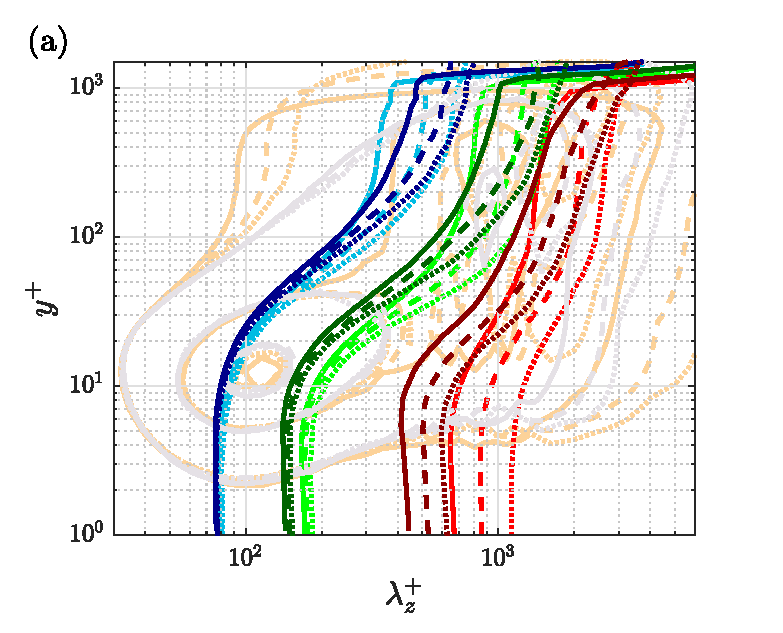
\includegraphics[width=0.49 \textwidth]{specMCE_uu_ltau_ltau.eps}
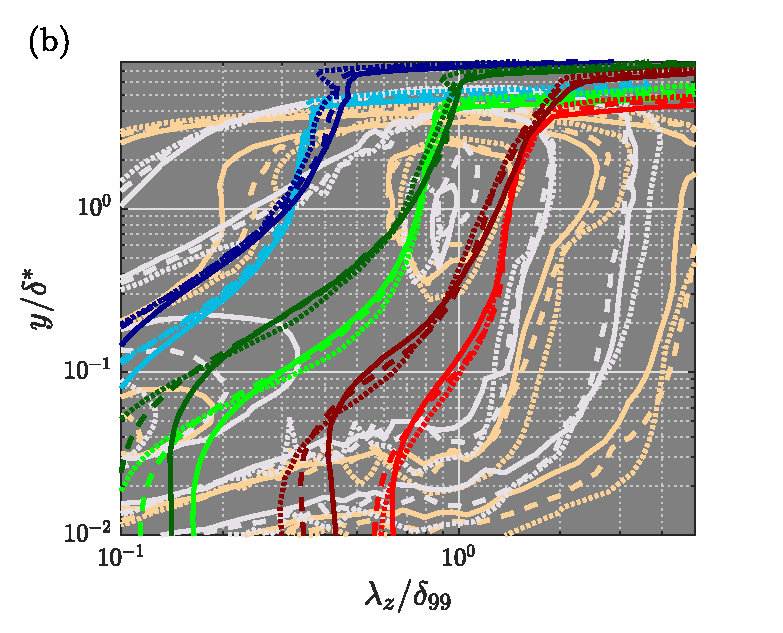
\includegraphics[width=0.49 \textwidth]{specMCE_uu_dstar_d99.eps}
\caption{ \label{fig:inner_kPSDz} Contours of the premultiplied spanwise power-spectral density of the streamwise RS, (a) scaled with the friction velocity, $k_z\phi_{uu}/u_{\tau}^2$, and (b) scaled with the edge velocity, $k_z\phi_{uu}/U_{e}^2$, both shown in lighter colors according to Table~\ref{tab:PGcases}. Contours taken at energy levels 0.5, 1.8 and 3.2 in panel (a). The levels for contours in panel (b) are: $[0.4, 1.2, 3] \times 10^{-3}$. The blue, green and red lines represent the size of the scales where the accumulated energy from the smallest scales add up to 20, 50 and $80\%$ of the total RS at that wall-normal location, respectively; for these lines, the light colors are used for the APG, while the dark colors are used for the ZPG.}
\end{figure}

% \subsection{Outer region}

In the outer region of the APG TBL it is also possible to differentiate two regions, the first one containing small energetic scales and another region of large scales surrounding the spectral outer peak.
As observed in Fig.~\ref{fig:peaks}(b), using $y/\delta^*$ and $\lambda_z/\delta_{99}$, the premultiplied spectral outer peak collapses for both APG and ZPG at different Reynolds numbers, although the value of the spectral outer peak is higher in the APG than for the ZPG case.
Since the outer scaling with $U_e^2$ yields a good collapse of $\overline{u^2}$ in the outer region for both cases \cite{Pozuelo_JFM_22}, the premultiplied spectra will be scaled with $U_e^2$, and the contours will be taken at a similar energy level.


%----------------------------------------------------------------------------------
%----------------------------------------------------------------------------------

In Fig.~\ref{fig:inner_kPSDz}(b), the outer spectral peak at different Reynolds numbers are located around the same location for both APG and ZPG and its scales are of a similar size, however, the APG energizes the scales around that peak.
% \rev{
% Wide scales of size $\lambda_z=4 \delta_{99}$ extend their influence across the TBL in the APG, while for the same energetic level the scales in the ZPG are of size $\lambda_z=3 \delta_{99}$.
% }
The large scales above $y=\delta^*$ contribute in a similar proportion to the RS (up to their respective $\delta_{99}/\delta^*$ values), independently of the Reynolds number or the APG (see red and green lines), while some differences start to be observed for the smaller scales (blue lines), since the APG contains more energy in smaller scales in this region. 
Between $y=0.1\delta^*$ and $y=\delta^*$, the large scales contribute in a similar way at different Reynolds numbers, but the relevance of the large scales is greater in the APG than in the ZPG. 
\begin{figure}
\centering
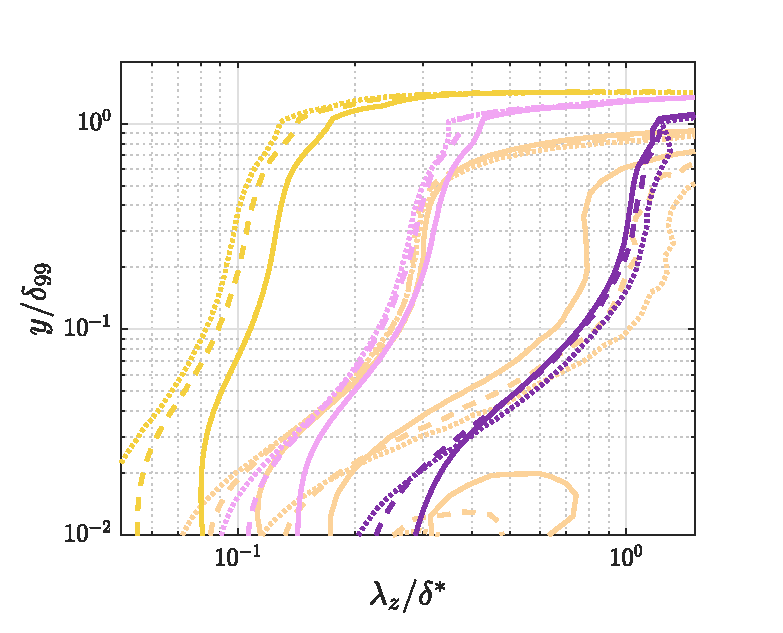
\includegraphics[width=0.6 \columnwidth]{specMCE_uu_d99_dstar.eps}
\caption{ \label{fig:cont_cumsum_d99_dstar} Outer-scaled premultiplied power-spectral density of the streamwise RS, $k_z\phi_{uu}/U_e^2$. Contours taken at $[0.4, 1.2, 3] \times 10^{-3}$. The yellow, pink and purple lines are the MCE contours at 0.1, 2.2 and $15\%$, respectively.}
\end{figure}

In Fig.~\ref{fig:cont_cumsum_d99_dstar} we focus on the energetic small scales in the outer region of the APG. The energetic contours of $k_z\phi_{uu}/U_e^2$ are taken at the same levels as those in Fig.~\ref{fig:inner_kPSDz}(b). The smaller energy level (light orange lines) collapses for scales of size $\lambda_z \approx 0.3 \delta^*$ where the MCE is $2.2\%$ (pink lines). 
Less energetic contours were investigated to assess whether the scaling $\lambda_z/\delta^*$ is still valid for smaller scales. This resulted in a behaviour similar to what the yellow MCE contours show. Other scalings such as $\delta_{99}$ lead to further distancing of the energy contours for scales $\lambda_z < 0.3\delta^*$.

This is the first time that the energy of the small scales in the outer region of an APG TBL is assessed in detail in terms of their scaling and their MCE.
From the MCE contours it can be observed that the smallest scales in the outer region add up to $2.2\%$ below $\lambda_z = 0.3 \delta^*$ and $15\%$ for scales $\lambda_z < \delta^*$.
Although the energy contour levels around $\lambda_z = \delta^*$ do not exhibit any collapse with the Reynolds number, the MCE purple lines do, implying that the scales between $\lambda_z = 0.3 \delta^*$ and $\lambda_z = \delta^*$ (pink and purple lines) contribute in a similar way to the total RS.
The lack of collapse in the energy contours of the premultiplied spectra would in principle indicate that there is no similarity between the scales in this region; however, the MCE reveals that their marginal contribution is in fact very similar.

This small-scale energy in the outer region is not present in the ZPG, and the MCE contours do not exhibit any collapse, thus we did not include those contours in Fig.~\ref{fig:cont_cumsum_d99_dstar}.
%----------------------------------------------------------------------------------
%----------------------------------------------------------------------------------
The Reynolds shear stress was also analysed. Its spectra in the near-wall region also scales in viscous units and even exhibits an inner peak in both APG and ZPG located at $y^+ \simeq 25$ and $\lambda_z^+ \simeq 105$. The energy level is similar in APG and ZPG using $u_{\tau}^2$. 
The Reynolds shear-stress spectrum also develops an outer spectral peak in both APG and ZPG, which is centered around $y/\delta^*=1.4$ and $\lambda_z/\delta_{99} = 0.9$. The energy of the outer spectral peak in the APG is almost twice the energy contained in its inner peak, while in the ZPG the values of the energy in its inner and outer peaks is similar.